\section{Structural Health Monitoring}

\subsection{Definition}

According to  \citet{balageas2010}, the \gls*{shm} main purpose is to provide, during the life of a structure,  a diagnosis of: the state of the constituent material; the different parts of the structure; and the full assembly of each part that makes the structure as a whole. 
It is an improved way to make non-destructive evaluation.
It can be applied in several areas such as civil infrastructure, like bridges and buildings; aerospace, like airplanes and spaceships; and mechanical, like machines.

\begin{figure}[H]
    \centering
    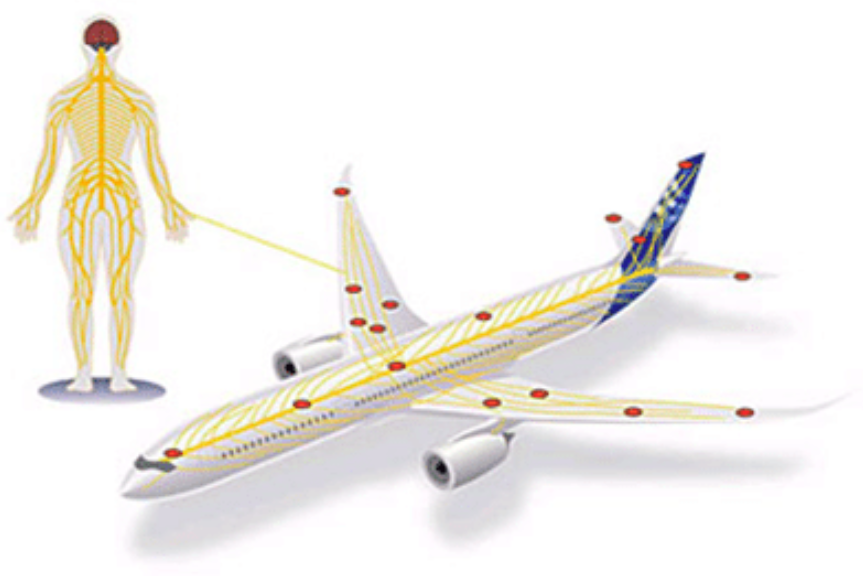
\includegraphics[width=0.6\textwidth]{figures/2methodology/shm/smh_nervous_system.png}
    \caption[SHM and human nervous system analogy]{\gls*{shm} and human nervous system analogy. Source: \citet{blanckenstein2015}}
    \label{fig:shm_nervous_system}
\end{figure}

It also can be associated as an analogy to the human nervous system, as shown in the \cref{fig:shm_nervous_system}. Just like the sensors send a signal to the central processor, the human 
senses send a signal to the brain to make the recognition of what is happening.

\subsection{Brief History}

The history goes back to the 1960s, when researches\(\ldots\) 

\begin{equation}
    \mathcal{L}\{f(x)\} = \lim_{\theta\to 0^+} \int_{\theta}^{\infty} f(x)\,\exp(-st) \, dt
\end{equation}